\documentclass[xcolor=table]{beamer}
\usepackage{beamerthemesplit}
\usepackage{wrapfig}
\usetheme{SPbGU}
\usepackage{pdfpages}
\usepackage{amsmath}
\usepackage{cmap} 
\usepackage[T2A]{fontenc} 
\usepackage[utf8]{inputenc}
\usepackage[english]{babel}
\usepackage{indentfirst}
\usepackage{amsmath}
\usepackage{tikz}
\usepackage{multirow}
\usepackage[noend]{algpseudocode}
\usepackage{algorithm}
\usepackage{algorithmicx}
\usepackage{fancyvrb}
\usetikzlibrary{shapes,arrows}
%usepackage{fancyvrb}
%\usepackage{minted}
%\usepackage{verbments}

\newtheorem{mytheorem}{Theorem}
\renewcommand{\thealgorithm}{}


\beamertemplatenavigationsymbolsempty

\title[F\# OpenCL C TP]{F\# OpenCL C Type Provider}
%\subtitle[YaccConstructor]{Parsing techniques for graph analysis}
% То, что в квадратных скобках, отображается в левом нижнем углу. 
\institute[JetBrains Research]{
JetBrains Research, Programming Languages and Tools Lab  \\
Saint Petersburg University
}

% То, что в квадратных скобках, отображается в левом нижнем углу.
\author[Semyon Grigorev]{Kirill Smirenko, \textbf{Semyon Grigorev}}

\date{September 27, 2018}

\definecolor{orange}{RGB}{179,36,31}

\begin{document}
{
\begin{frame}[fragile]
  \begin{tabular}{p{3.5cm} p{5.5cm} p{1cm}}
   \begin{center}
      
\includegraphics[height=1.5cm]{pictures/jetbrainsResearch.pdf}
    \end{center}
    &
    \begin{center}
      
\includegraphics[height=1.5cm]{pictures/icfplogo.png}
    \end{center}
    &
    \begin{center}
      
\includegraphics[height=1.5cm]{pictures/SPbGU_Logo.png}
    \end{center} 
  \end{tabular}
  \titlepage
\end{frame}
}

\begin{frame}[fragile]
  \transwipe[direction=90]
  \frametitle{GPGPU}
  \begin{minipage}[m]{0.40\linewidth}
\raisebox{-0.5\totalheight}{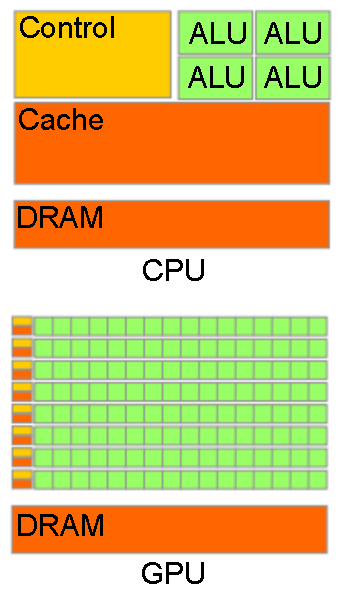
\includegraphics[height=0.85\textheight]{pictures/cpu_gpu.pdf}}
\end{minipage}\hfill
\begin{minipage}[m]{0.6\linewidth}
General purpose computations on graphical processor units
\begin{itemize}
      \item (Almost) SIMD architecture 
      \item Huge amount of ``simple'' ALUs on single chip
      \item Initially for computer graphic/games etc
      \item Good choice for big data processing   
\end{itemize}

\end{minipage}

\end{frame}

\begin{frame}[fragile]
  \transwipe[direction=90]
  \frametitle{General purpose applications of GPGPU}
  \begin{itemize}
    \item Initially for scientific computations
    \begin{itemize}
      \item Physics
      \item Math
      \item Chemistry
    \end{itemize}
    \item But more and more for applications
      \begin{itemize} 
        \item Finance/Banking
        \item Data Analytics and Data Science (Hadoop, Spark ...)
        \item Security analytics (log processing)
        \item Some ``scientific computations'' today are daily-used applications (bioinformatics, chemistry , \dots)
      \end{itemize}
  \end{itemize}
\end{frame}

\begin{frame}
  \transwipe[direction=90]
  \frametitle{High level languages and GPGPU}
\begin{minipage}[m]{0.45\linewidth}
Low-level platforms and languages for GPGPU programming
\begin{itemize}
\item NVIDIA CUDA: Cuda C, Cuda Fortran
\item \textbf{OpenCL: OpenCL C}
\end{itemize}
\end{minipage}\hfill
\begin{minipage}[m]{0.45\linewidth}
High-level platform and languages for applications
\begin{itemize}
      \item C++
      \item Python, Haskell, OCaml, \dots
      \item JVM: Java, Scala, \dots 
      \item \textbf{.NET: C\#, F\#, \dots}
\end{itemize}
\end{minipage}

\pause
\vspace{1cm}
\center{\huge{Interaction is a problem!}}
\end{frame}

\begin{frame}[fragile]
  \transwipe[direction=90]
  \frametitle{Possible solutions}
  \begin{itemize}
  \item Translation of high-level language to GPGPU specific one
    \begin{itemize}
  \item[+] Useful features of host language for GPGPU programming (type safety, etc)
  \item[-] High performance GPGPU programs is inherently low-level
  \end{itemize}
  \item Reusing of existing GPGPU libraries
      \begin{itemize}
  \item[+] GPGPU optimized solution in low-level language
  \item[?] We need automatic generation of ``well-typed'' bindings
  \end{itemize}

  \end{itemize}
\end{frame}

\begin{frame}[fragile]
  \transwipe[direction=90]
  \frametitle{Brahma.FSharp}
  \begin{itemize}
  \item F\# quotations to OpenCL C translator
  \item Runtime
      \begin{itemize}
        \item Comand queue
        \item Execution context management
        \item Memory management
        \item F\# aliases for OpenCL-specific functions
      \end{itemize}

  \end{itemize}
\end{frame}

\begin{frame}
  \transwipe[direction=90]
  \frametitle{F\# type providers}
\begin{itemize}
 \item Compile-time metaprogramming technique for compile-time types creation
 \begin{itemize}
  \item Type provider is a ``function which constructs type''
 \end{itemize}
 \item Design-time features in IDE
 \begin{itemize}
   \item Completion
   \item Type information
 \end{itemize}
 \item Used for type-safe integration of external data with ``fixed schema''
 \begin{itemize}
   \item Type providers for XML, JSON, INI, etc
   \item R, SQL, etc type providers
 \end{itemize}
\end{itemize}

\end{frame}


\begin{frame}[fragile]
  \transwipe[direction=90]
  \frametitle{Example of INI type provider}

\small{
\begin{verbatim}
[Section1]
intSetting = 2
stringSetting = stringValue
[Section2]
floatSetting = 1.23
boolSetting = true
anotherBoolSetting = False
emptySetting =
stringWithSemiColonValue = DataSource=foo@bar;UserName=blah 
\end{verbatim}
}
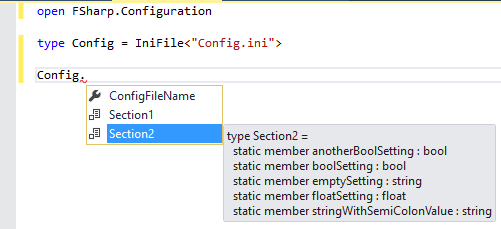
\includegraphics[width=0.6\textwidth]{pictures/INIExample.png}

\end{frame}

\begin{frame}
  \transwipe[direction=90]
  \frametitle{OpenCL C type provider}
\begin{itemize}
\item We want to construct type-safe wrapper for given Open!!!!
\item OpenCL standard declares source-level distribution with ``in place'' compilation
\begin{itemize}
\item[+] We can work with source code (text), not with binaries
\item[--] ``Existing library'' is a set of files includes *.h files
\end{itemize}
\item Functions signatures processing should be enough for basic integration
\end{itemize}
\end{frame}
 
\begin{frame}
  \transwipe[direction=90]
  \frametitle{OpenCL C type provider: architecture}
    
  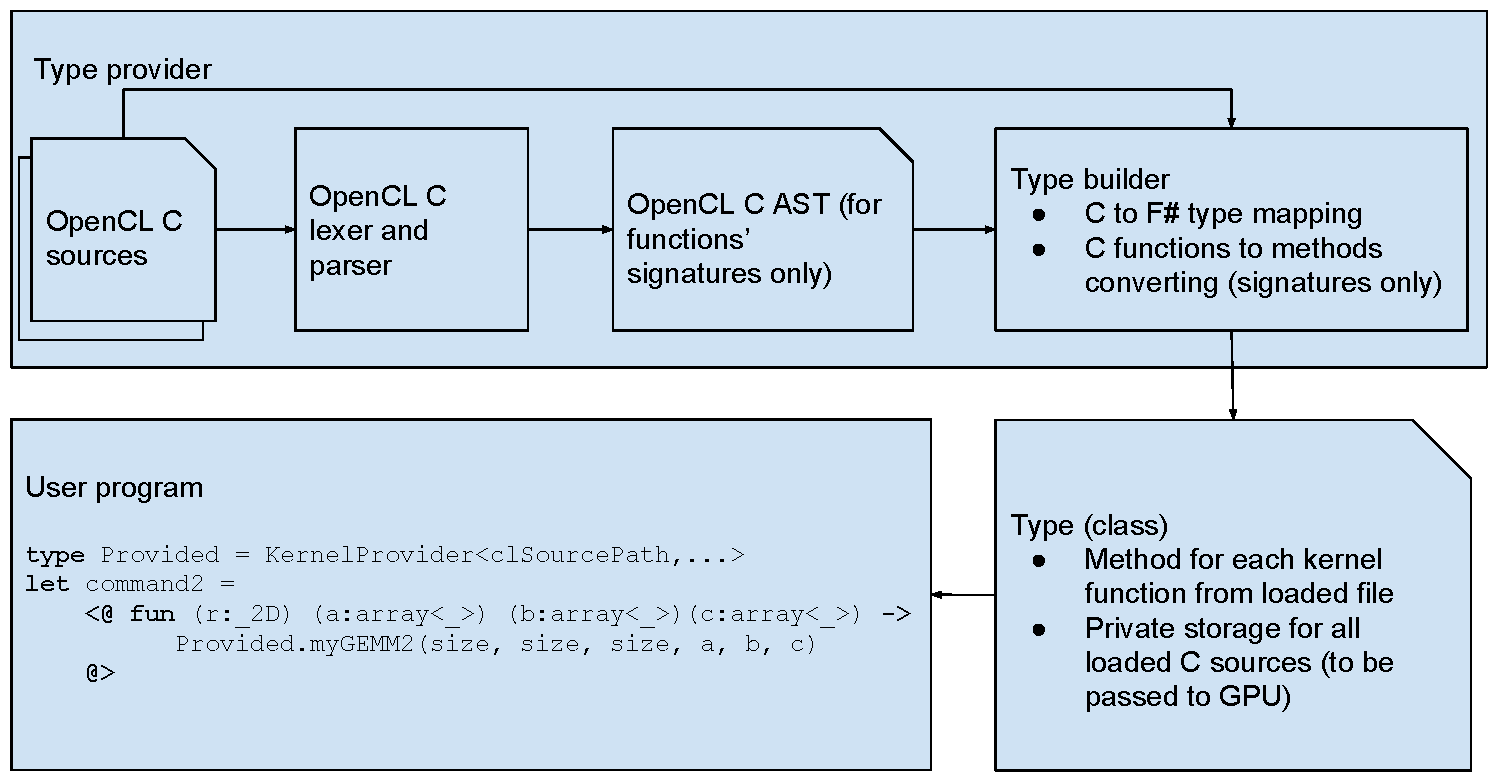
\includegraphics[width=0.95\textwidth]{pictures/OpenCL_C_TP.pdf}
  \\
  \pause
  \center{Yes, it is typical type provider}
\end{frame}

\begin{frame}
  \transwipe[direction=90]
  \frametitle{Limitations}
\begin{itemize}
\item Only (small) subset of OpenCL C
 \begin{itemize}
 \item h files is not supported
 \item preprocessor is not supported
 \item only small subset of syntax is supported
  \end{itemize}
\item Very simple C to F\# type mapping
\item \dots
\end{itemize}

\end{frame}

            
\begin{frame}
  \transwipe[direction=90]
  \frametitle{Examples}         
  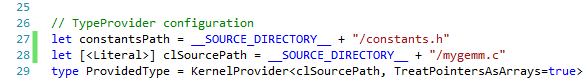
\includegraphics[width=0.95\textwidth]{pictures/smpl1.png}
  \\
  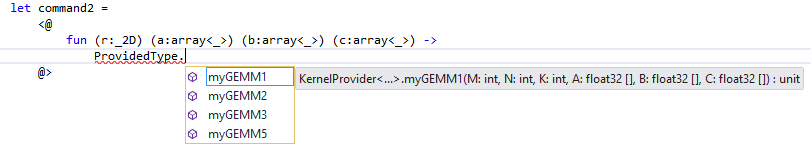
\includegraphics[width=0.95\textwidth]{pictures/smpl2.png}
  \\
  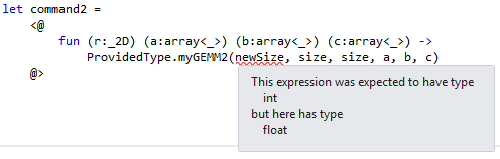
\includegraphics[width=0.95\textwidth]{pictures/smpl3.png}
\end{frame}     

\begin{frame}
  \transwipe[direction=90]
  \frametitle{Future work}         
\begin{itemize}
\item Improve OpenCL C support
\begin{itemize}
\item Lexer and parser
\item Translator 
\item Types mapping
\item Headers files processing
\item \dots
\end{itemize}
\item Unify kernels on client side
\begin{itemize}
\item Currently native Brahma.FSharp's kernel and kernel loaded by type provider are different 
types
\end{itemize}
\item Improve mechanism of kernels composition
\end{itemize}
\end{frame}     
            
            
\begin{frame}
  \transwipe[direction=90]
  \frametitle{Summary}         
\begin{itemize}
\item F\# OpenCL C type provider
\begin {itemize}
\item Type-safe integration of existing OpenCL C code in F\# applications
\item Prototype with limitations
\end{itemize}
\vspace{1cm}
\item Source code on GitHub: \url{https://github.com/YaccConstructor/Brahma.FSharp}
\item Package on NuGet: \url{https://www.nuget.org/packages/Brahma.FSharp/}
\end{itemize}
\end{frame}           
            
\begin{frame}
\transwipe[direction=90]
\frametitle{Contact Information}
\begin{itemize}
  \item Semyon Grigorev: \href{mailto:s.v.grigoriev@spbu.ru}{s.v.grigoriev@spbu.ru}
  \item Kirill Smirenko: \href{mailto:k.smirenko@gmail.com}{k.smirenko@gmail.com}
\end{itemize}
\begin{itemize}
  \item Brahma.FSharp: \href{https://github.com/YaccConstructor/Brahma.FSharp}{https://github.com/YaccConstructor/Brahma.FSharp}
\end{itemize}
\hspace{2cm}
\center{\huge{Thanks!}}
\end{frame}
\end{document}
